\documentclass[12pt,a4paper,openright,twoside]{report}


\usepackage[british]{babel}
\usepackage[utf8]{inputenc}


\usepackage{fancyhdr}
\usepackage{indentfirst}
\usepackage{graphicx}
\usepackage{newlfont}
\usepackage{xcolor}


\usepackage{amssymb}
\usepackage{amsmath}
\usepackage{latexsym}
\usepackage{amsthm}


\oddsidemargin=30pt 
\evensidemargin=20pt
\hyphenation{sil-la-ba-zio-ne pa-ren-te-si}
\pagestyle{fancy}\addtolength{\headwidth}{20pt}
\renewcommand{\chaptermark}[1]{\markboth{\thechapter.\ #1}{}}
\renewcommand{\sectionmark}[1]{\markright{\thesection \ #1}{}}
\rhead[\fancyplain{}{\bfseries\leftmark}]{\fancyplain{}{\bfseries\thepage}}
\cfoot{}
\linespread{1.3}

% Style theorem boxes

\theoremstyle{plain}
\newtheorem{prop}{Proposition}
\newtheorem{defin}[prop]{Definition}
\newtheorem{intdef}[prop]{(Intuitive) Definition}

\theoremstyle{definition}
\newtheorem{rem}[prop]{Remark}
\newtheorem{ex}[prop]{Example}


%%%%%%%%%%%%%%%%%%%%%%%%% DEDICATION %%%%%%%%%%%%%%%%%%%%%%%%%%%%%%%%%%%%%%%

\begin{document}

\begin{titlepage}
\thispagestyle{empty}                   
\topmargin=6.5cm                        
\raggedleft                             
\large                                  
                                       
\em                                     
To my beloved\\
Benedetta                   
\newpage                                

\clearpage{\pagestyle{empty}\cleardoublepage}
\end{titlepage}
\pagenumbering{roman}


            




%%%%%%%%%%%%%%%%%%%%%%% INTRODUCTION %%%%%%%%%%%%%%%%%%%%%%%%%%%%%%

\chapter*{Introduction}   
\addcontentsline{toc}{chapter}{Introduction}
\rhead[\fancyplain{}{\bfseries Introduction}]{\fancyplain{}{\bfseries\thepage}}\lhead[\fancyplain{}{\bfseries\thepage}]{\fancyplain{}{\bfseries Introduction}}




  \textcolor{blue}{Machine learning literature is exploding in size and complexity, but most solutions found are ad hoc, there is little communication between different subfields, and there is a large research debt. Category theory can solve these problems.  \cite{shieblerCategoryTheoryMachine2021}.}

  \textcolor{blue}{Talk about the origins of category theory and its "rise to power" as a common language that aims to unite different fields of knowledge.}
    
  \textcolor{blue}{Discuss the purpose of this work: a beginner-friendly survey of categorical approaches to neural networks, causal models, and interpretability.}





%%%%%%%%%%%%%%%%%%%%%%% ITALIAN TRANSLATION OF THE INTRODUCTION %%%%%%%%%%%%%%%%%%%%%%%%%%%%%%


\chapter*{Introduzione}
\addcontentsline{toc}{chapter}{Introduzione}
\rhead[\fancyplain{}{\bfseries Introduzione}]{\fancyplain{}{\bfseries\thepage}}\lhead[\fancyplain{}{\bfseries\thepage}]{\fancyplain{}{\bfseries Introduzione}}





  \textcolor{blue}{Traduzione italiana dell'introduzione.}







%\clearpage{\pagestyle{empty}\cleardoublepage}


%%%%%%%%%%%%%%%%%%%%%%%%%%%%% TABLE OF CONTENTS %%%%%%%%%%%%%%%%%%%%%%%%%%%%%%

\tableofcontents
\rhead[\fancyplain{}{\bfseries\leftmark}]{\fancyplain{}{\bfseries\thepage}} \lhead[\fancyplain{}{\bfseries\thepage}]{\fancyplain{}{\bfseries Table of Contents}}
%\clearpage{\pagestyle{empty}\cleardoublepage}

\listoffigures                         
%\clearpage{\pagestyle{empty}\cleardoublepage}


\listoftables                           
%\clearpage{\pagestyle{empty}\cleardoublepage}





%%%%%%%%%%%%%%%%%%%%%%%%% CATEGORICAL TOOLKIT %%%%%%%%%%%%%%%%%%%%%%%%%%%%%


\chapter{Categorical Toolkit}
\lhead[\fancyplain{}{\bfseries\thepage}]{\fancyplain{}{\bfseries\rightmark}}
\pagenumbering{arabic}



\textcolor{blue}{Brief introduction to category theory and the categorical toolkit used in the following sections. As each kind of category is introduced we shall also introduce appropriate string diagrams.}



  \section{Basics of Category Theory}


  \textcolor{blue}{Definition of category.}
  \textcolor{blue}{Definition of functor.}
  \textcolor{blue}{Definition of natural transformation.}
  \textcolor{blue}{Definition of 2-category.}


  \section{Various Families of Categories}

  \subsection{Monoidal Categories}

  \textcolor{blue}{Definition of monoidal category.}
  \textcolor{blue}{Definition of Cartesian category.}
  \textcolor{blue}{Expand on the properties of Cartesian categories. In particular, expand on the existence of copy maps.}
  \textcolor{blue}{Definition of left-additive category.}
  \textcolor{blue}{Definition of Cartesian left-additive category.}




  \subsection{Differential Categories}

  The recent rise in AI techniques was only possible because of advancements in automatic differentiation (AD) techniques. Differentiation in machine learning is usually carried out in Euclidean spaces $\mathbb{R}^n$, but is worth considering more abstract settings because the techniques used in gradient-based learning can be greatly generalized. For instance, \cite{wilsonReverseDerivativeAscent2021a} demonstrated that gradient-based learning can take place in the context of Boolean circuits.


  We consider two abstract settings for differentiation: Cartesian differential categories (first introduced in \cite{bluteDifferentialCategories2006}) and Cartesian reverse differential categories (first introduced by \cite{cockettReverseDerivativeCategories2019}). The former is a setting where forward derivatives of morphisms can be taken, while the latter is a setting where reverse derivatives can be taken. We shall only give intuitive definitions for the sake of brevity; rigorous definition which account of all the necessary axioms can be found in \cite{cockettReverseDerivativeCategories2019}.

  \begin{intdef}[Cartesian differential category]
    A Cartesian differential category (CDR) $\mathcal{C}$ is a Cartesian left-additive category where a differential combinator $\mathrm{D}$ is defined. Such differential combinator must take a morphism $f: A \to B$ and return a morphism $\mathrm{D}[f]: A \times A \to B$, which is known as the derivative of $f$. The combinator $\mathrm{D}$ must satisfy a number of axioms. 
  \end{intdef}

  \begin{intdef}[Cartesian reverse differential category]
    A Cartesian reverse differential category (CRDC) $\mathcal{C}$ is a Cartesian left-additive category where a reverse differential combinator $\mathrm{R}$ is defined. Such reverse differential combinator must take a morphism $f: A \to B$ and return a morphism $\mathrm{R}[f]: A \times B \to A$, which is known as the reverse derivative of $f$. The combinator $\mathrm{R}$ must satisfy a number of axioms. 
  \end{intdef}

  
  The aforementioned axioms make sure that $\mathrm{R}$ and $\mathrm{D}$ satisfy the properties expected from derivative and reverse derivative. In particular, a differential combinator satisfies a chain rule (see figure ADDIM), whereas a reverse differential combinator satisfies a reverse chain rule (see figure ADDIM).

  
  \begin{ex}
    $\mathbf{Smooth}$ is a both a CDC and a CRDC. In fact, if $\mathcal{J}_f$ is the Jacobian matrix of a smooth morphism $f$,
    \[\mathrm{D}[f]: (x,v) \mapsto \mathcal{J}_f(x)v\]
    and
    \[\mathrm{R}[f]: (x,y) \mapsto \mathcal{J}_f(x)^Ty\]
    induce well-defined combinators $\mathrm{D}$ and $\mathrm{R}$. This is only a partial coincidence, as it is shown in \cite{cockettReverseDerivativeCategories2019} that CRDCs are always CDCs under a canonical choice of differential combinator. The converse, however, is generally false.
  \end{ex}



  \subsection{Lenses}

  Lenses are a mathematical construct used to model bidirectional flows of information\footnote{The theory of optics generalizes lenses to a much wider family of constructs that model these same bidirectional flows. See \cite{rileyCategoriesOptics2018}.}. Such flows are extremely important in machine learning as a machine learning model needs both to carry out a computation and to update its parameters based on the training data.

  \begin{defin}[Lenses]
    Let $\mathcal{C}$ be a Cartesian category. We define $\mathbf{Lens}(\mathcal{C})$ as the category constituted by the following objects and morphisms.
    An object of $\mathbf{Lens}(\mathcal{C})$ is a pair $\begin{pmatrix} A \\ A' \end{pmatrix}$ of objects in $\mathcal{C}$; 
    A $\begin{pmatrix} A \\ A' \end{pmatrix} \to \begin{pmatrix} B \\ B' \end{pmatrix}$ morphism (or lens) is a pair $\begin{pmatrix} f \\ f^* \end{pmatrix}$ of morphisms of $\mathcal{C}$ such that $f: A \to B$ and $f^*: A \times A'$. $f$ is known as get part of the lens $\begin{pmatrix} f \\ f^* \end{pmatrix}$, whereas $f^*$ is known as get part. Given a pair $\begin{pmatrix} A \\ A' \end{pmatrix}$, the associated identical lens is $\begin{pmatrix} 1_A \\ \pi_1 \end{pmatrix}$. Lens composition is illustrated by ADDIM.
  \end{defin}

  Lenses can be represented using the language string diagrams (see \cite{cruttwellDeepLearningParametric}), both in compact form and in expanded form.


  It is important to note the following (see \cite{cruttwellDeepLearningParametric}):
  
  \begin{prop}
    If $\mathcal{C}$ is a Cartesian category, $\mathbf{Lens}(\mathcal{C})$ is a monoidal category under the monoidal product $\begin{pmatrix} A \\ A' \end{pmatrix} \otimes \begin{pmatrix} B \\ B' \end{pmatrix} = \begin{pmatrix} A \times B \\ A' \times B' \end{pmatrix}$.
  \end{prop}

  Another important result from \cite{cruttwellDeepLearningParametric} is (according the formulation found in \cite{shieblerCategoryTheoryMachine2021}):

  \begin{prop}
    If $\mathcal{C}$ is a CRDC, there exists a canonical Cartesian left-additive functor $R_\mathcal{C}$ which embeds $\mathcal{C} \to \mathbf{Lens}(\mathcal{C})$. Such functor maps objects as $A \mapsto \begin{pmatrix}A \\ A\end{pmatrix}$ and maps morphisms as $f \mapsto \begin{pmatrix}f \\ \mathrm{R}[f]\end{pmatrix}$.
  \end{prop}

  \begin{rem}
    Consider the put map of the composition of two lenses, as in figure ADDIM. As \cite{shieblerCategoryTheoryMachine2021} notes, there is a striking resemblance between the form that such put map takes and the reverse chain rule that holds in a CRDC. This similarity will be important for modelling neural networks as lenses. 
  \end{rem}




  \subsection{The $\mathbf{Para}$ Construction}

  In machine learning, it is often necessary to work with parameters. Although lenses can model bidirectional flow, they don't afford us the machinery needed to work with such parameters. The $\mathbf{Para}$ construction allows us to overcome such limit. For the sake of simplicity, we shall only examine the case where parameters and values are taken from the same category $\mathcal{C}$ (as in \cite{cruttwellDeepLearningParametric}). A more general $\mathbf{Para}$ construction is described in \cite{shieblerCategoryTheoryMachine2021}, where actegories are used to handle a much wider choice of possible parameters.

  \begin{intdef}[$\mathbf{Para}(\mathcal{C})$]
    Let $(\mathcal{C},I,\otimes)$ be a symmetric monoidal category. Then, we define $\mathbf{Para}(\mathcal{C})$ as the $2$-category whose components are as follows.
    \begin{itemize}
      \item The $0$-cells are the objects of $\mathcal{C}$.
      \item The $1$-cells are pairs $(P,f): A \to B$, where $P \in \mathcal{C}$ and $f: P \otimes A \to B$.
      \item The $2$-cells come in the form $r: (P,f) \to (Q,g)$, where $r: P \to Q$ is a morphism in $\mathcal{C}$. $r$ must also satisfy a naturality condition.
      \item The $1$-cell identity on $A$ in $\mathbf{Para}(\mathcal{C})$ is $(I,1_A)$.
      \item The $2$-cell identity on $(P,f)$ in $\mathbf{Para}(\mathcal{C})$ is $1_P$.
      \item The $1$-cell composition law is
        \[(P,f) ; (Q,g) = (Q \otimes P, Q \otimes f ; g.\]
      \item The $2$-cell composition law is the same as the $\mathcal{C}$ composition law.
    \end{itemize}
     
  \end{intdef}

  The intuition behind the definition above is the following: the $1$ cells are parametric maps, whereas the $2$ cells are reparametrisations.
  It is quite handy to represent such cells using the string diagram notation illustrated in figure ADDIM.
  
  
  It is shown in \cite{cruttwellDeepLearningParametric} that $\mathbf{Para}(\mathcal{C})$ is natural with respect to $\mathcal{C}$. In other words, as emphasized in \cite{shieblerCategoryTheoryMachine2021},
  
  \begin{prop}
    If $\mathcal{C}$ and $\mathcal{D}$ are symmetric monoidal categories and $F: \mathcal{C} \to \mathcal{D}$ is a symmetric monoidal functor, then  there is a canonical $2$-functor 
    \[\mathbf{Para}(F): \mathbf{Para}(\mathcal{C}) \to \mathbf{Para}(\mathcal{D}).\]
  \end{prop}






  %\begin{figure}[h]
  %  \begin{center}                         
  %    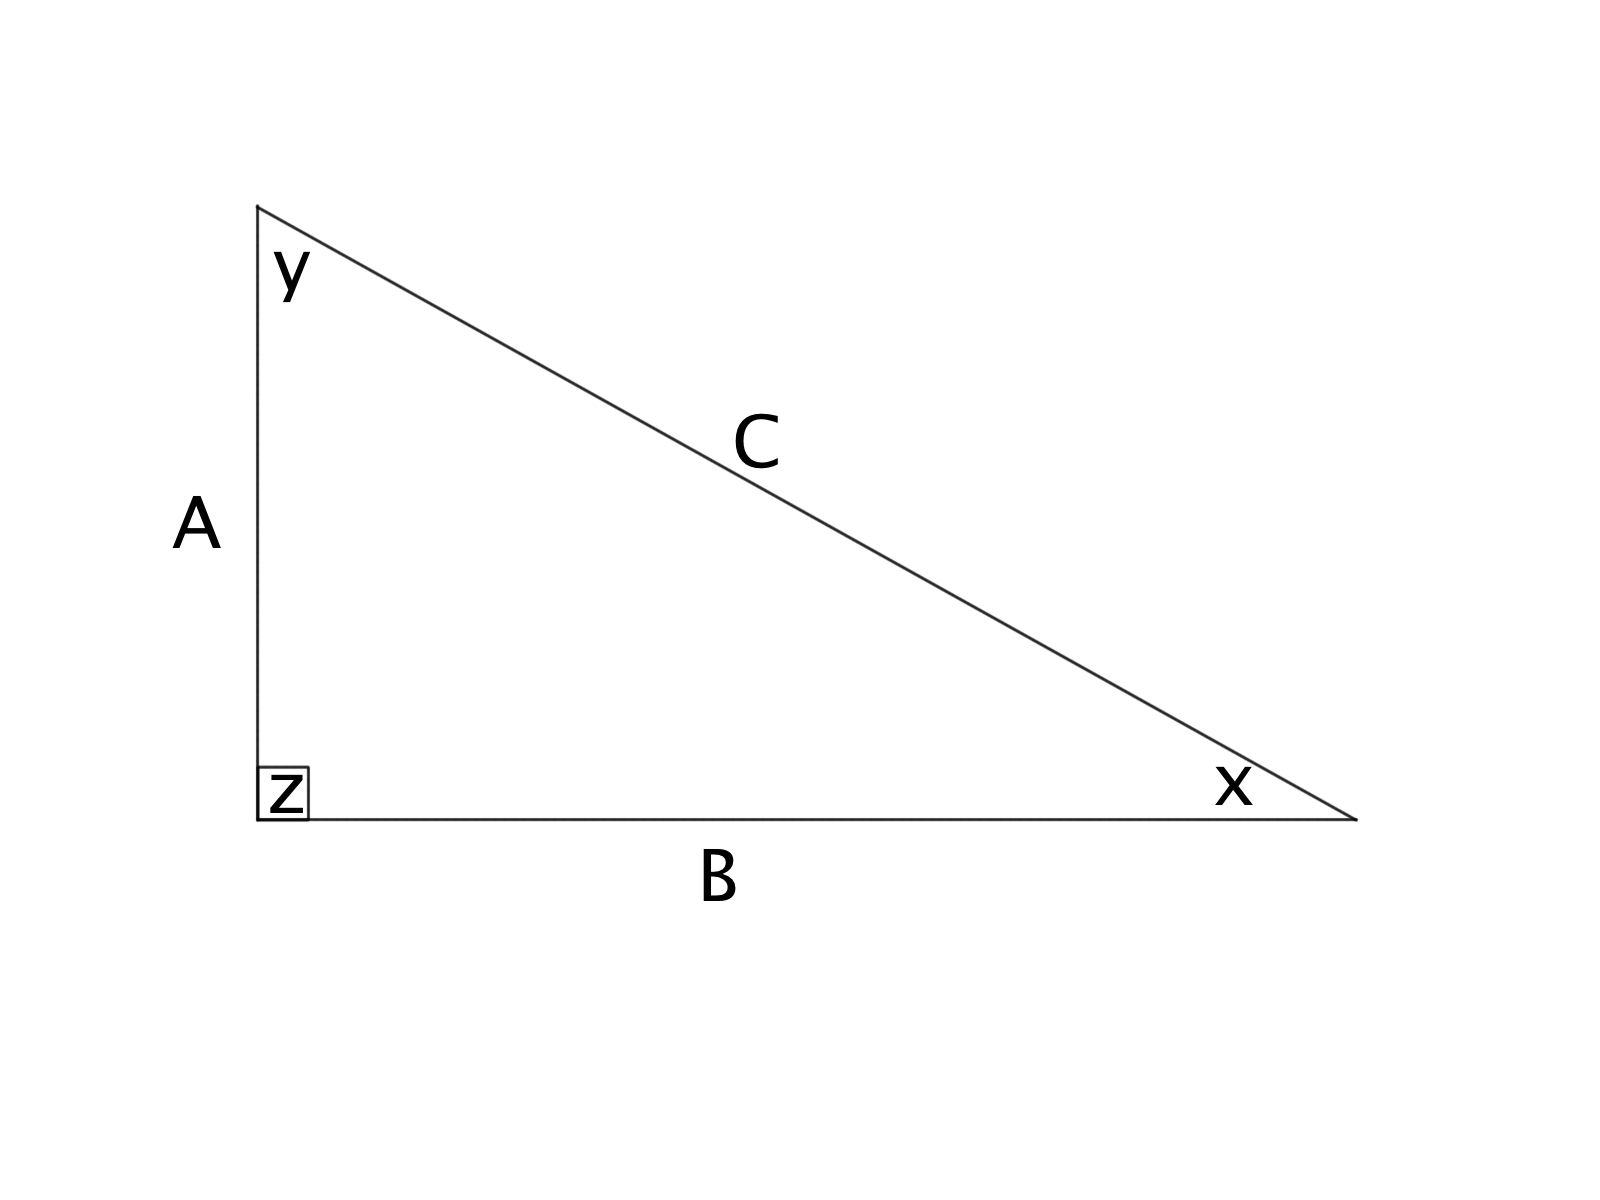
\includegraphics[width=5cm]{figures/triangle.jpg}
  %    \caption[Placeholder]{Placeholder figure.}\label{fig:first}
  %  \end{center}
  %\end{figure}

  %\begin{table}[h]                        
  %  \begin{center}                          
  %    \begin{tabular}{r|c|c}                  
  %      \hline \hline                           
  %      $(1,1)$ & $(1,2)$ & $(1,3)$\\           
  %      \hline                                  
  %      $(2,1)$ & $(2,2)$ & $(2,3)$\\           
  %      \hline                                  
  %      $(3,1)$ & $(3,2)$ & $(3,3)$\\
  %      \hline \hline                           
  %    \end{tabular}
  %    \caption[Placeholder Table]{Placeholder table.}\label{tab:uno}
  %  \end{center}
  %\end{table}



%%%%%%%%%%%%%%%%%%%%%%% CATEGORICAL APPROACHES TO NNS %%%%%%%%%%%%%%%%%%%%%%%%%%%


\chapter{Categorical Approaches to Neural Networks}
\lhead[\fancyplain{}{\bfseries\thepage}]{\fancyplain{}{\bfseries\rightmark}}




\textcolor{blue}{Brief summary of the chapter.}





\section{Neural Networks as Parametric Lenses}

\textcolor{blue}{Parametric lenses allow us to represent neural networks so that we can model both forward and backward propagation at the same time. This representation is compositional, and the learning iteration can also be represented \cite{cruttwellDeepLearningParametric}.}






\subsection{Neural Networks as Parametric Maps}





\subsection{Neural Networks as Parametric Lenses}





\subsection{Learning with Parametric Lenses}

\textcolor{blue}{Show that loss functions and optimizers can be represented as parametric lenses. Show that such components can be combined to actually model learning. Show that the learning iteration itself can be handled like this \cite{cruttwellDeepLearningParametric}.}

\textcolor{blue}{Parametric lenses can be successfully applied to software development \cite{cruttwellDeepLearningParametric}.}








%\clearpage{\pagestyle{empty}\cleardoublepage}

%%%%%%%%%%%%%%%%%%%%%%%%%%%%%% CONCLUSIONS %%%%%%%%%%%%%%%%%%%%%%%%%%%%%%%%%%%

\chapter*{Conclusions}
\rhead[\fancyplain{}{\bfseries
Conclusions}]{\fancyplain{}{\bfseries\thepage}}
\lhead[\fancyplain{}{\bfseries\thepage}]{\fancyplain{}{\bfseries Conclusions}}
\addcontentsline{toc}{chapter}{Conclusions} 










%%%%%%%%%%%%%%%%%%%%%%%%%%%%%%%%%%%%% BIBLIOGRAPHY %%%%%%%%%%%%%%%%%%%%%%%%%%%%%%

\bibliographystyle{alpha}
\bibliography{references}
\rhead[\fancyplain{}{\bfseries \:Bibliography}]{\fancyplain{}{\bfseries\thepage}} 
\addcontentsline{toc}{chapter}{Bibliography}



% \clearpage{\pagestyle{empty}\cleardoublepage}



%%%%%%%%%%%%%%%%%%%%%%%%%%%%%%%%%%%%%%% ACKNOWLEDGEMENTS %%%%%%%%%%%%%%%%%%%%%%%%%%%

\chapter*{Acknowledgements}

\thispagestyle{empty}

  Placeholder 



\end{document}
